\subsubsection{評価ルール}
全体的な評価ルールは置換モデルの時と変わらない.

\begin{itemize}
\item 複合式の部分式を評価する
\item オペレーターをオペランドの部分式の値に適用する
\end{itemize}

しかし, 環境モデルではプロシージャを適用する時, 評価ルールが変わってくる.
環境モデルにおいて, プロシージャはコードと環境へのポインタの組み合わせで定義される.
プロシージャを作る唯一の方法は, \lstinline{lambda}式を評価することである.
例えば,

\begin{lstlisting}[basicstyle=\footnotesize]
(define (square x) (* x x))
\end{lstlisting}
が
\begin{lstlisting}[basicstyle=\footnotesize,caption=]
(define square (lambda (x) (* x x)))
\end{lstlisting}
として評価されるので, グローバル環境で\lstinline{square}に
\lstinline{lambda}式をバインドする.

\begin{figure}[h]
  \centering
  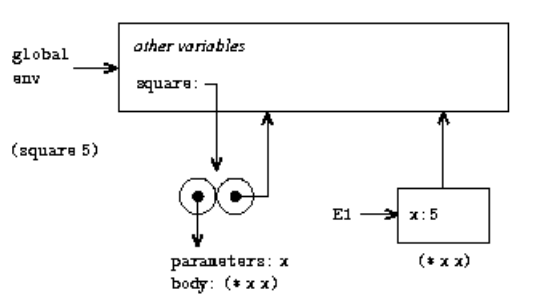
\includegraphics[height=5cm,width=12cm]{imgs/square_env.png}
  \caption{\label{fig:square-env}グローバル環境での\lstinline{(square 5)}の実行}
\end{figure}


環境モデルでは, プロシージャの適用は以下の2つのルールでまとめることができる.
\begin{itemize}
\item プロシージャは\lstinline{lambda}式を評価することによって作成される.
  プロシージャは環境を持つので, コードと環境へのポインタの組み合わせとして定義される.
\item プロシージャの適用の時, 新しいフレームが作成される.
  そのフレームの環境はプロシージャの環境となる.
  新しく作られたフレームで仮引数が実引数にバインドされる.
\end{itemize}

図\ref{fig:square-env}で実行例を示す.